\documentclass[12pt]{article}
\usepackage{graphicx}
%\documentclass[journal,12pt,twocolumn]{IEEEtran}
\usepackage[none]{hyphenat}
\usepackage{graphicx}
\usepackage{listings}
\usepackage[english]{babel}
\usepackage{graphicx}
\usepackage{caption}
\usepackage[parfill]{parskip}
\usepackage{hyperref}
\usepackage{booktabs}
%\usepackage{setspace}\doublespacing\pagestyle{plain}
\def\inputGnumericTable{}
\usepackage{color}                                            %%
    \usepackage{array}                                            %%
    \usepackage{longtable}                                        %%
    \usepackage{calc}                                             %%
    \usepackage{multirow}                                         %%
    \usepackage{hhline}                                           %%
    \usepackage{ifthen}
\usepackage{array}
\usepackage{amsmath}   % for having text in math mode
\usepackage{parallel,enumitem}
\usepackage{listings}
\lstset{
language=tex,
frame=single,
breaklines=true
}
 
%Following 2 lines were added to remove the blank page at the beginning
\usepackage{atbegshi}% http://ctan.org/pkg/atbegshi
\AtBeginDocument{\AtBeginShipoutNext{\AtBeginShipoutDiscard}}
%
%New macro definitions
\newcommand{\mydet}[1]{\ensuremath{\begin{vmatrix}#1\end{vmatrix}}}
\providecommand{\brak}[1]{\ensuremath{\left(#1\right)}}
\providecommand{\norm}[1]{\left\lVert#1\right\rVert}
\newcommand{\solution}{\noindent \textbf{Solution: }}
\newcommand{\myvec}[1]{\ensuremath{\begin{pmatrix}#1\end{pmatrix}}}
\let\vec\mathbf
\begin{document}
\begin{center}
\enlargethispage{-4cm}
\title{\textbf{Straight Lines}}
\date{\vspace{-5ex}} %Not to print date automatically
\maketitle
\end{center}
\setcounter{page}{1}
\section*{11$^{th}$ Maths - Chapter 10}
This is Problem-1 from Exercise 10.4
\begin{enumerate}
\item Find the values of $k$ for which the line $(k-3)x-(4-k^2)y+k^2-7k+6=0$ is
\begin{enumerate}
\item Parallel to the $x$-axis
\item Parallel to the $y$-axis
\item Passing through the origin
\end{enumerate}

\solution
Given line is
\begin{align}
(k-3)x-(4-k^2)y+k^2-7k+6=0 \label{eq:1}
\end{align}
this equation can be expressed in the form of 
\begin{align}
\vec{n}^{\top}\vec{x}=c \label{eq:2}
\end{align}
\begin{align}
\text{ where }
\vec{n} = \myvec{k-3\\-4+k^2} , c  = -k^2+7k-6
\end{align}
then \eqref{eq:1} can be expressed as
\begin{align}
\myvec{k-3 & -4+k^2}\vec{x} &=-k^2+7k-6\label{eq:4}
\end{align}
\begin{enumerate}
%part-1
    \item Parallel to $x$-axis
    
The normal vector of $x$-axis is given by
\begin{align}
\myvec{0\\1}
\end{align}
Equating the $\vec{n}$ to the normal vector of $x$-axis
\begin{align}
\myvec{k-3\\-4+k^2} &=\alpha\myvec{0\\1}\\
0 &=\alpha\myvec{0\\1}\myvec{-4+k^2\\k-3}\\
k &=3
\end{align}
Substituting the value of $k$ in \eqref{eq:4} then equation of line parallel to $x$-axis is given by
\begin{align}
        \myvec{0 & 5}\vec{x} &=6
\end{align}
The line parallel to $x$-axis is shown is Figure \eqref{fig:Fig1}

\begin{figure}[!h]
\begin{center}
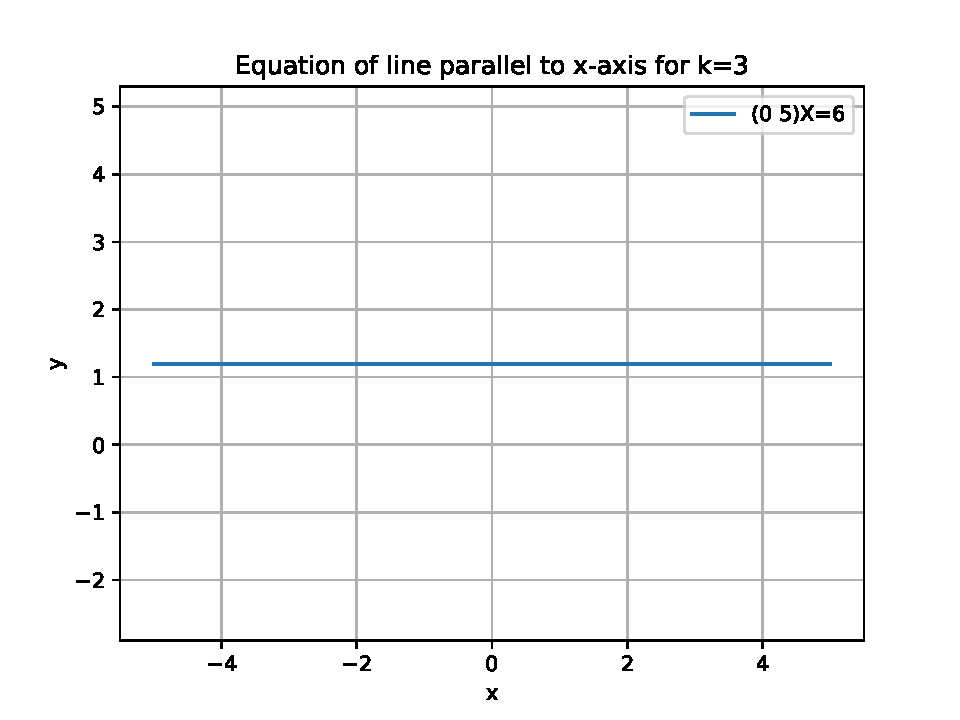
\includegraphics[width=\columnwidth]{figs/fig1.pdf}
\end{center}
\caption{}
\label{fig:Fig1}
\end{figure}
%part-2

\item Parallel to $y$-axis

The normal vector of $y$-axis is given by
\begin{align}
\myvec{1\\0}
\end{align}
Equating the $\vec{n}$ to the normal vector of $y$-axis
\begin{align}
\myvec{k-3\\-4+k^2} &=\alpha\myvec{1\\0}\\
0 &=\alpha\myvec{1\\0}\myvec{-4+k^2\\k-3}\\
k &=\pm2
\end{align}
Substituting the value of $k$ in \eqref{eq:4} then equation of line parallel to $y$-axis is given by
\begin{align}
\text{for } k &=2\\
        \myvec{-1 & 0}\vec{x} &=4\\
\text{for } k &=-2\\
        \myvec{-5 & 0}\vec{x} &=-24
\end{align}
The line parallel to $y$-axis is shown is Figure \eqref{fig:Fig2}

\begin{figure}[!h]
\begin{center}
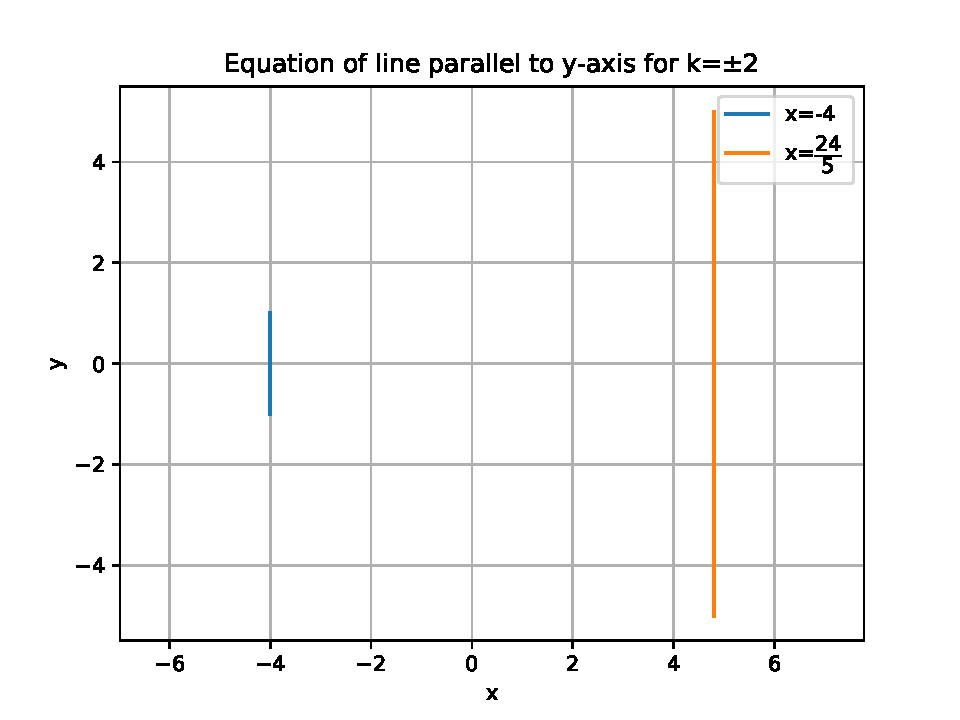
\includegraphics[width=\columnwidth]{figs/fig2.pdf}
\end{center}
\caption{}
\label{fig:Fig2}
\end{figure}

%part-3
\item Passing through the origin

When line is passing through origin $(0,0)$ then $x$ and $y$ coordinates are equal to $0$, then 
\begin{align}
    \myvec{k-3 & -4+k^2}\vec{x} &= -k^2+7k-6\\
    0 &=-k^2+7k-6\\
   \implies k &=1 \text{ or } k=6
\end{align}
Substituting the value of $k$ in \eqref{eq:4} then equation of line parallel to $y$-axis is given by
\begin{align}
\text{for } k &=1\\
        \myvec{-2 & -3}\vec{x} &=0\\
\text{for } k &=6\\
       \myvec{3 & 32}\vec{x} &=0
\end{align}
The line passing through origin $(0,0)$ is shown is Figure \eqref{fig:Fig3}

\begin{figure}[!h]
\begin{center}
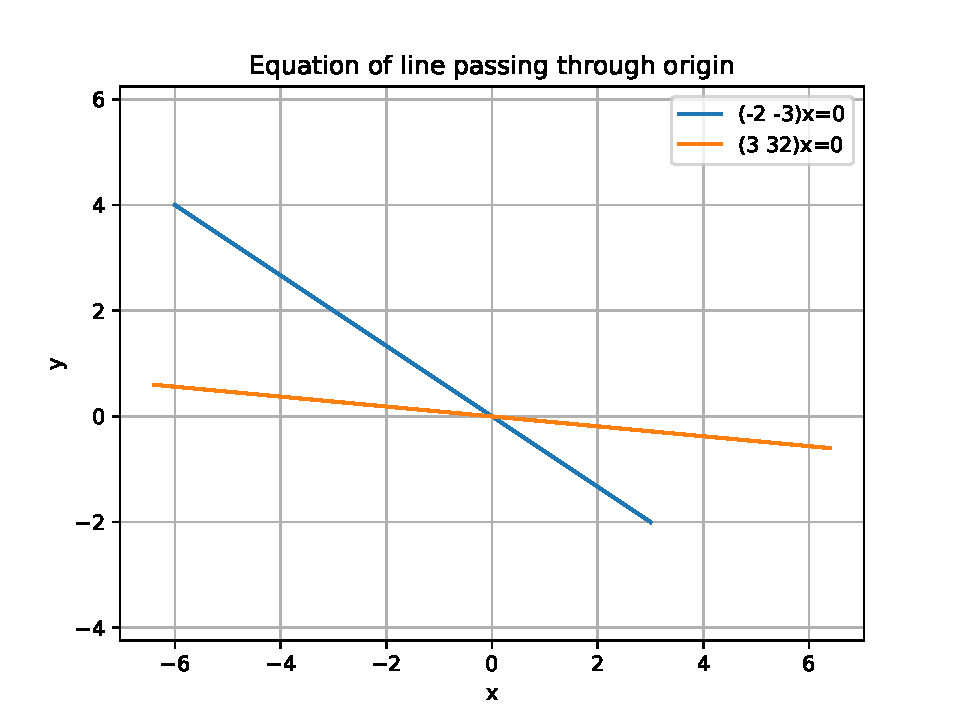
\includegraphics[width=\columnwidth]{figs/fig3.pdf}
\end{center}
\caption{}
\label{fig:Fig3}
\end{figure}
\end{enumerate}
\end{enumerate}
\end{document}